\documentclass{beamer}
\usepackage[utf8]{inputenc}
\usetheme{Berlin}

\title{Conception et développement multi-lots /  multi-équipes\\ \emph{application à la supervision à distance d'une ligne de conditionnement temps réel}}
\author{Hexanôme 4203\\Etienne \textsc{Brodu} Martin \textsc{Richard} Maxime \textsc{Gaudin} Monica \textsc{Golumbeanu} Paul \textsc{Adenot} Yoann \textsc{Rodière}}

\begin{document}

	\begin{frame}
		\titlepage
	\end{frame}

\section{introduction}
	\begin{frame}
		\begin{itemize}	
			\item Lampes
			\item Impression des étiquettes %Charge des imprimantes
			\item Journal d'exploitation
			\item Client Windows
			\item Erreurs et Anomalies
			\item Protocole
			%TODO Est-ce bien nécessaire de tout détailler ?
		\end{itemize}
	\end{frame}

	\begin{frame}
		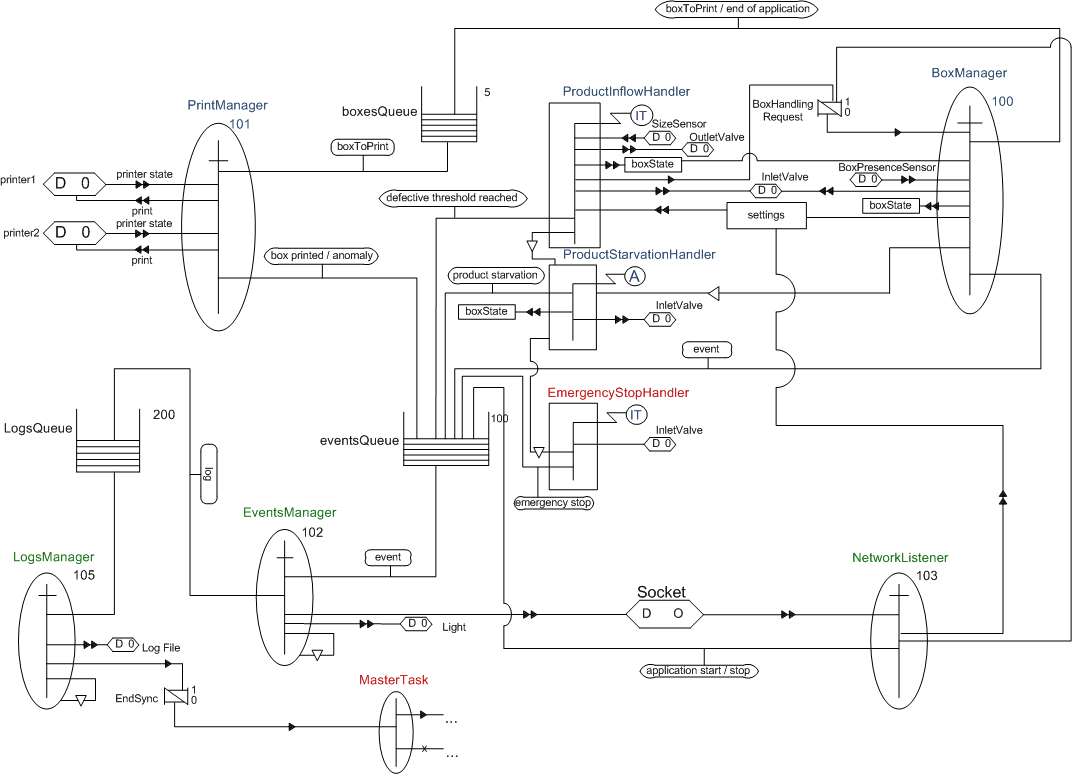
\includegraphics[width=\textwidth]{../../SchemasLCG/schemaGlobal.png}
		%TODO Découpage en lot fonctionnel.
	\end{frame}

	\begin{frame}
		IHM du poste distant
		connection
	\end{frame}

	\begin{frame}
		IHM du poste distant
		configuration
	\end{frame}

	\begin{frame}
		IHM du poste distant
		log
	\end{frame}

	\begin{frame}
		IHM du poste distant
		erreur \/ warning
	\end{frame}

\section{Binôme 1}
	\begin{frame}
		LCG détaillé et complet en mode simulation
	\end{frame}

	\begin{frame}
		justification des choix effectués pour la simulation 
	\end{frame}

\section{Binôme 2}
	\begin{frame}
		LCG détaillé et complet en mode simulation
	\end{frame}

	\begin{frame}
		justification des choix effectués pour la simulation  
	\end{frame}

\section{Binôme 3}
	\begin{frame}
		LCG détaillé et complet en mode simulation
	\end{frame}

	\begin{frame}
		justification des choix effectués pour la simulation 
	\end{frame}

\section{Intégration}
	\begin{frame}
		Intégration
		\begin{itemize}
			\item démarche
			\item plan
			\item tests
			\item resultats
		\end{itemize}
		%TODO
	\end{frame}

	\begin{frame}
		démonstration de vos réalisations
		%TODO démonstration externe au slides ?
	\end{frame}

	\begin{frame}
		bilan du projet
		\begin{itemize}
			\item auto-critique
			\item améliorations possibles
			\item points forts/faibles
			\item difficultés rencontrées ...
		\end{itemize}
		%TODO
	\end{frame}

\end{document}

